
\documentclass[sigconf]{acmart}

\AtBeginDocument{%
  \providecommand\BibTeX{{%
    Bib\TeX}}}


\setcopyright{acmlicensed}
\copyrightyear{2025}
\acmYear{2025}
\acmDOI{https://doi.org/10.1145/3715669.3726816.}
\acmConference[ETRA2025]{ACM Symposium on Eye Tracking Research \& Applications}{May 26--29,
  2018}{Tokyo, Japan}

\acmISBN{978-1-4503-XXXX-X/2018/06}


%%
%% Submission ID.
%% Use this when submitting an article to a sponsored event. You'll
%% receive a unique submission ID from the organizers
%% of the event, and this ID should be used as the parameter to this command.
%%\acmSubmissionID{123-A56-BU3}

%%
%% For managing citations, it is recommended to use bibliography
%% files in BibTeX format.
%%
%% You can then either use BibTeX with the ACM-Reference-Format style,
%% or BibLaTeX with the acmnumeric or acmauthoryear sytles, that include
%% support for advanced citation of software artefact from the
%% biblatex-software package, also separately available on CTAN.
%%
%% Look at the sample-*-biblatex.tex files for templates showcasing
%% the biblatex styles.
%%

%%
%% The majority of ACM publications use numbered citations and
%% references.  The command \citestyle{authoryear} switches to the
%% "author year" style.
%%
%% If you are preparing content for an event
%% sponsored by ACM SIGGRAPH, you must use the "author year" style of
%% citations and references.
%% Uncommenting
%% the next command will enable that style.
%%\citestyle{acmauthoryear}

% Add this to reduce the space between figures and text
\setlength{\textfloatsep}{10pt}
\setlength{\floatsep}{10pt}
\setlength{\intextsep}{10pt}


\begin{document}


\title{Floating Captions: Eyetracking-based Context-aware Captioning System for Immersive VR Contents}

\author{Kosuke Shimizu}
\authornote{Both authors contributed equally to this research.}
\orcid{1234-5678-9012}
\affiliation{%
  \institution{University of Tsukuba}
  \city{Tsukuba}
  \state{Ibaraki}
  \country{Japan}
}
\email{shimizu@ai.iit.tsukuba.ac.jp}

\author{Shohei Komatsu}
\authornotemark[1]
\orcid{1234-5678-9012}
\affiliation{%
  \institution{University of Tokyo}
  \city{Bunkyo}
  \state{Tokyo}
  \country{Japan}
}
\email{komatsu-shohei@g.ecc.u-tokyo.ac.jp}



\author{Hidenori Watanave}
\affiliation{%
  \institution{University of Tokyo}
  \city{Bunkyo}
  \state{Tokyo}
  \country{Japan}
}
\email{hwtnv@iii.u-tokyo.ac.jp}

\renewcommand{\shortauthors}{Shimizu and Komatsu et al.}


\begin{abstract}
Exhibiton captions or didactic panel in museum play a crucial role for providing information. However, the separation of exhibits and exhibit description hinders the viewer's appreciation, especially in contexts that require a sense of realism. Our goal is to integrate captioning into exhibits in a non-obstructive manner. Our system creates a circular 'gaze point within the exhibit's space, and when the user fixes their gaze on it for specific periods of time, a caption is subsequently displayed. This system is a context-aware method of presenting information in response to the user's gaze, and reduces the number of captions displayed concurrently, facilitating an uninterrupted immersive viewing experience.
\end{abstract}

\begin{CCSXML}
<ccs2012>
  <concept>
    <concept_id>10003120.10003121.10003126</concept_id>
    <concept_desc>Human-centered computing~Virtual reality</concept_desc>
    <concept_significance>500</concept_significance>
  </concept>
  <concept>
    <concept_id>10003120.10003121.10003122</concept_id>
    <concept_desc>Human-centered computing~Interaction techniques</concept_desc>
    <concept_significance>300</concept_significance>
  </concept>
  <concept>
    <concept_id>10002978.10002991.10002992</concept_id>
    <concept_desc>Information systems~Multimedia information systems</concept_desc>
    <concept_significance>100</concept_significance>
  </concept>
</ccs2012>
\end{CCSXML}


\ccsdesc[500]{Human-centered computing~Virtual reality}
\ccsdesc[300]{Human-centered computing~Interaction techniques}
\ccsdesc[100]{Human-centered computing~Empirical studies in HCI}
\ccsdesc[100]{Information systems~Multimedia information systems}

\begin{teaserfigure}
  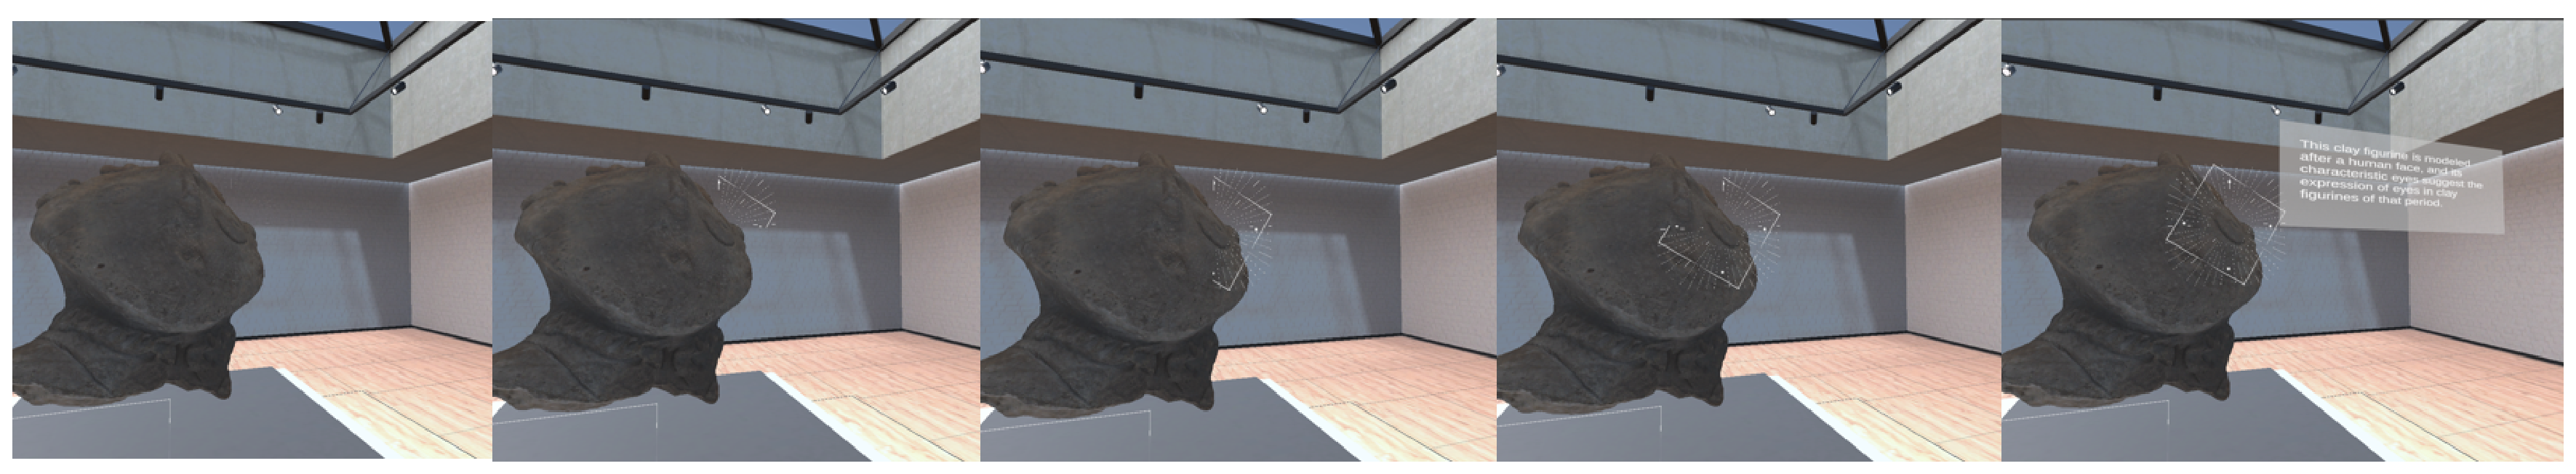
\includegraphics[width=\textwidth]{teaser.eps}
  \caption{The figure shows user’s dwell time, and description label is presented after detecting sufficient dwell time}
  \Description{The process of captioning.}
\end{teaserfigure}

\keywords{Context-Aware Captioning, Eye-tracking, Virtual Reality}
%% A "teaser" image appears between the author and affiliation
%% information and the body of the document, and typically spans the
%% page.


% \received{20 February 2025}
% \received[revised]{12 March 2009}
% \received[accepted]{5 June 2009}

%%
%% This command processes the author and affiliation and title
%% information and builds the first part of the formatted document.
\maketitle

\section{Introduction}
Descriptive caption in museum have long played a crucial role in providing additional information during the appreciation of cultural exhibits, artworks, or historical materials\cite{pedersen2017more}. As well as usual museums, virtual museums employ captions to improve accessibility and comprehension\cite{Dondi2023,ibrahim2018conceptual}. However, conventional captioning methods often require the placement of text separately from the exhibit itself, such as on static panels or overlays. This can inadvertently increase the cognitive load for viewers\cite{SWELLER1988257,GINNS2006511}.

% As captions become more extensive, viewers are forced to divide their attention between the visual content and the textual information\cite{GINNS2006511}.

This disruption impedes immersion and potentially diminishes the overall impact of the virtual experience.
%Swellerでcognitive loadの説明をしつつ,ginnsではextraneous cognitive loadについて触れる.学習に無関係な、完全に余計な負荷.

These challenges are especially salient in contexts where a sense of realism is paramount, such as when using 3D-scanned sites to capture the aftermath of disasters or conflicts. The authenticity and emotional engagement in these sites are central to the experience\cite{Komatsu2023,Komatsu2024}.%%小松さんのをcitationする.
Extensive on-screen text disrupts the atmosphere of historical or cultural significance. This can result in a shift of the viewer's focus from the scene's emotional weight, thereby undermining the core purpose of preserving an immersive environment conducive to deeper reflection and learning.
%% 執筆済み.

In order to address the aforementioned issues, a number of approaches have been developed to reduce visual clutter and cognitive burden. For example, Lu et al.\cite{Lu2021} developed a guidance method for virtual exhibits of long scrolls that automatically begin to display audio commentary and keywords when the user approaches a certain distance from a particular exhibit location. Also, it has been reported that users' ability to process information is improved by using world-fixed annotation, which links information to a specific place in the world, rather than screen-fixed annotation, which fixes information to the screen\cite{Dominic2020}. 

%% 文章量的におそらく必要ない
% GlanceAR, which fixes secondary information to the left and right sides of the head and allows the user to glance at the information in a left-right inverted motion of the head, has also been developed\cite{Lu2020}.
%% 執筆済み.ここではXRにおける情報提示についてちょっと触れる.

Eye-tracking technology is mature enough to use as an Input/Output interaction. Indeed, eye tracking has been utilized mainly in games, and Mutasim et al. created a system that combines button operations and gestures together with gaze to assist aiming in game operations\cite{Mutasim2021}. Andersson et al. have made systems to dynamically adjust the amount of information on the screen by automatically hiding visual elements of the heads-up display that the player is not looking at\cite{Andersson2020}. Eye tracking is beginning to be used in real museums. In museums where eye tracking is implemented, systems are already in place to track the user's gaze and provide feedback on how individuals view artwork after they leave the museum\cite{Dondi2023}. 
Current trends indicate that guiding attention and presenting information through eye gaze is considered a powerful means of enhancing the user experience, and UI methods are actively being evaluated to match the characteristics of Virtual Reality(VR)\cite{Hu2020}. These previous studies show that it is important to avoid adding unnecessary information to the user's view, to distribute captions in appropriate places, and to realize "presenting information when the user wants it".

In this paper, we propose a new gaze-based eye captioning system designed for virtual museum environments, with particular application to 3D reconstructions of disaster or war-affected sites. Our solution introduces a small circular "gaze point" within the virtual space, which displays a relevant caption only after the user has fixated on it for n seconds. This design aims to reduce the overwhelming volume of displayed text at any single moment and to integrate caption reading more seamlessly into the viewing experience. By avoiding large text panels or constant overlays, we seek to uphold immersion and maintain the emotional and historical authenticity of the reconstructed environment. 

\section{Method}
For the development of the system, we employed PICO 4 Enterprise (Bytedance Inc.) for eye tracking and VR viewing. The system was developed using Unity as the basic platform, with PICO Unity Integration SDK. In every second, eye tracking coordinate information is exported as a csv file, which is converted to coordinate positions in the user's HMD field of view in real time. The circular "gaze point" is designed to be visually subtle and is sized in proportion to the virtual object it corresponds to.  

For determining appropriate dwell time thresholds, we drew upon established research in eye-tracking interaction. Isomoto et al.\cite{Isomoto2023} have found that the dwell-time required for completing cognitive processes varies significantly depending on task complexity, and they revealed that complex image selection tasks required between 272.5ms and 835.8ms depending on viewer familiarity. Zhang et al.\cite{Zhang2011} investigated the speed-accuracy trade-off in dwell-based eye pointing tasks and found that dwell times below 200ms significantly increased error rates, while thresholds above 800ms were perceived as unnecessarily slow. Špakov and Miniotas demonstrated that dwell times between 600-800ms provided an optimal balance for most users in interactive contexts\cite{Spakov2004}. Following these prior works, in our virtual museum application, we determined that a relatively conservative threshold of 750ms would be appropriate given several considerations: First, museum content typically involves unfamiliar and complex visual material that requires cognitive processing. Second, accidental triggering of captions (the "Midas Touch" problem) would significantly disrupt the immersive experience we aim to preserve, particularly in emotionally significant reconstructions of disaster or conflict sites. 

\begin{figure}
    \centering
    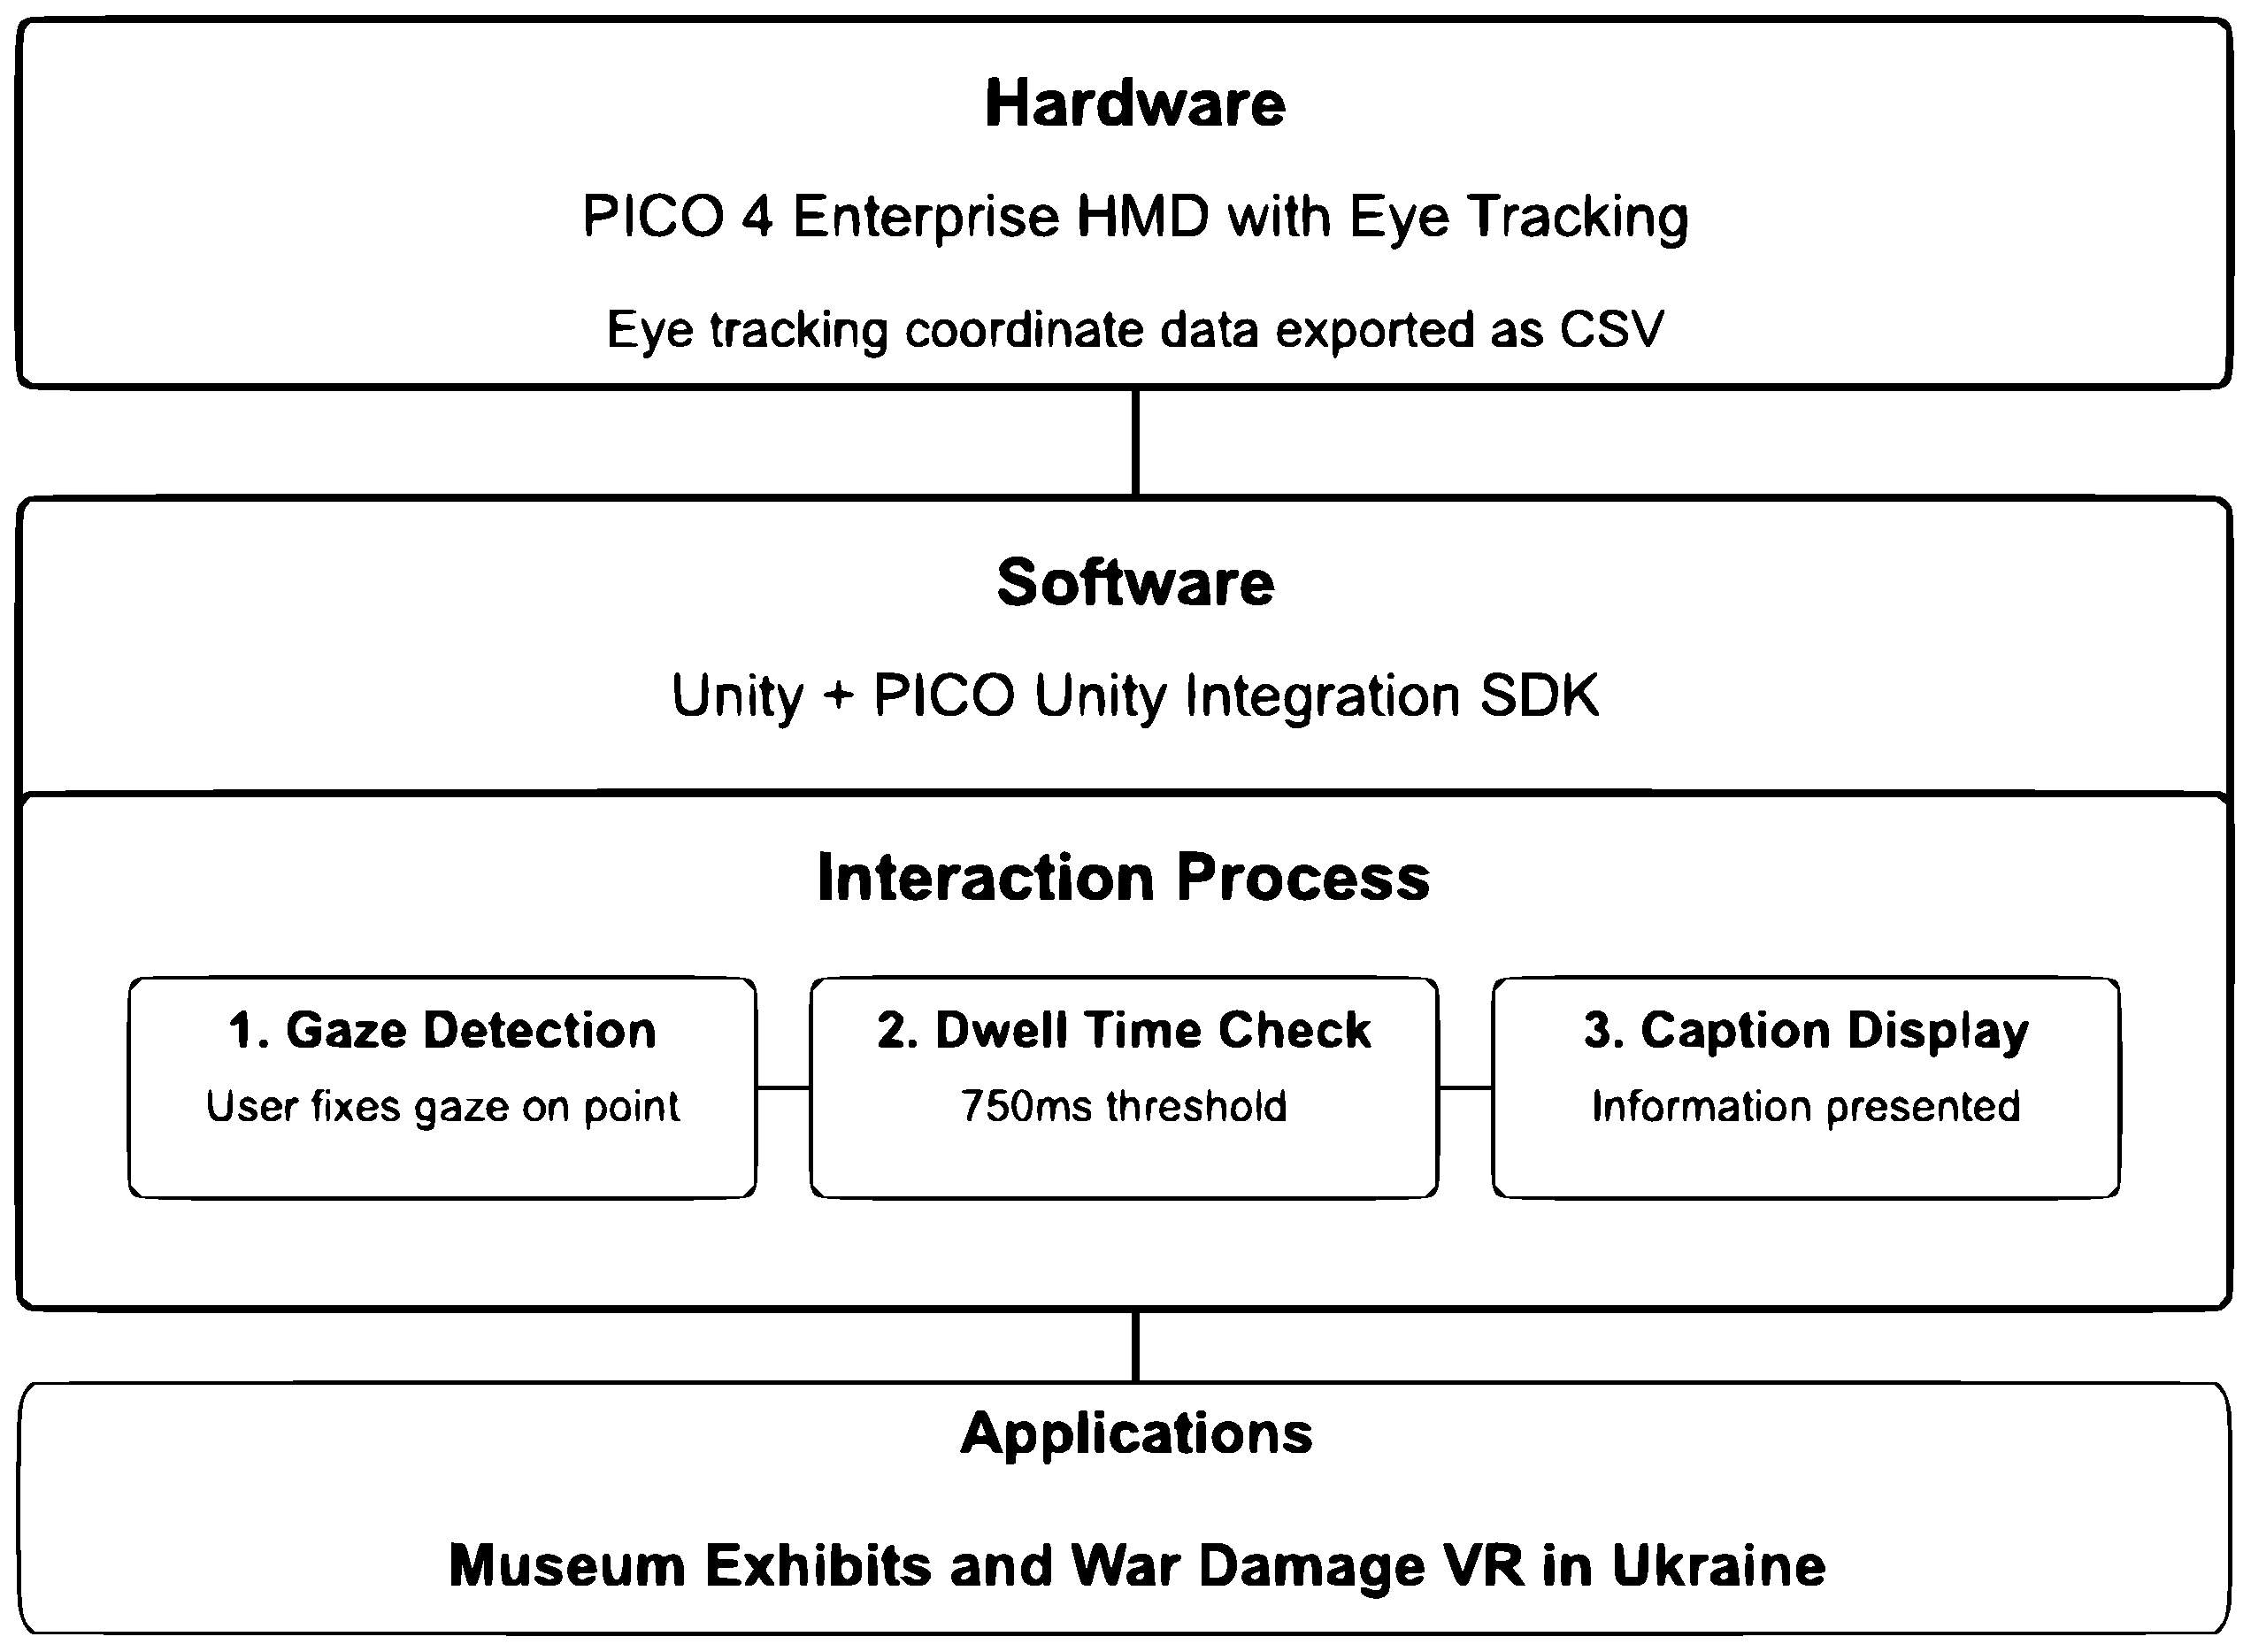
\includegraphics[width=0.8\linewidth]{Method.eps}
  \caption{System consists of }
  \label{fig:teaser}
  \Description{}
\end{figure}

\section{Demonstration}
%% 目視で再現することができます.
Two fields are available for the demonstration, and ten gaze points are available in each field. The first field imitates a digital museum, displaying 3D data of collection materials from the Matsudo City Museum(align open source 3D model of exhibits), and the appropriateness of the information presentation method is discussed. The second field features War Damage VR\cite{Komatsu2023}, an immersive experience of affected areas in Ukraine, and discusses whether the system will not interfere with the immersive experience. Since the War Disaster VR deals with content related to war, we will inform viewers about this sensitive content before the demonstration. This experience will subsequently stimulate a discussion regarding the method of information presentation in the Virtual Museum and the validity of the algorithm for information presentation using eye tracking. 

\begin{figure}
    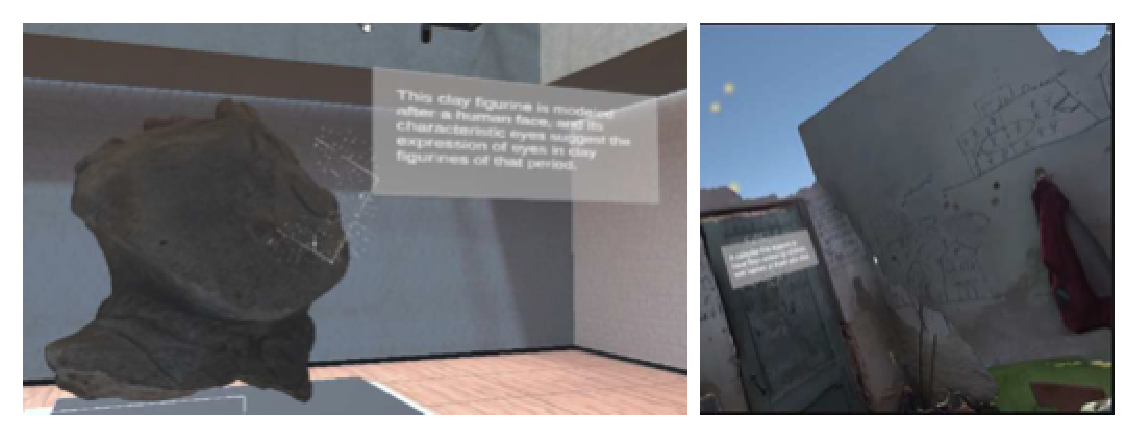
\includegraphics[width=0.8\linewidth]{demonstration.eps}
  \caption{Left figure shows the scene of captioning the description of Jo-mon earthenware; Right figure shows the scene in devastated area of Ukraine}
  \label{fig:teaser}
  \Description{Left figure shows the scene of captioning the description of Jo-mon earthenware; Right figure shows the scene in devastated area of Ukraine.}
\end{figure}
%% 松戸の博物館は Attribution-ShareAlike 4.0 International のCCなので使用可能である.https://sketchfab.com/3d-models/c31b4cb6b58645db8c1f898e426371b6


\section{Conclusion and Future Work}
In this paper, we present new context-aware information presentation system triggered by eye tracking. In the future, we will conduct rigorous testing of the system's impact on human cognition and measure how effectively this system preserves the VR viewing experience, including optimizing dwell time for caption presentation.


\begin{acks}
In this study, we received cooperation from BiPSEE Inc. for VR content production. The Matsudo City Museum provided the materials for the demonstration exhibits through sketchfab. Also, this work is supported by Fund for Digital Archives of War and Disasters, The University of Tokyo.
\end{acks}


\bibliographystyle{ACM-Reference-Format}
\bibliography{ref}

\end{document}
